\documentclass[a4paper,twoside]{IEEEtran}

\newcommand{\seminarteilnehmer}{Tim Budweg}
\newcommand{\seminartitel}{TODO: Der Titel Ihrer Seminararbeit}

% Löschen oder kommentieren Sie die folgenden beiden Zeilen aus,
% wenn Sie den Text in Englisch schreiben wollen.
\usepackage{german}
\usepackage[utf8]{inputenc}

\usepackage{graphicx}
\graphicspath{{figures/eps/}}
\usepackage{ dsfont }




\usepackage{amsmath}


\begin{document}

\title{\seminartitel}
\author{\seminarteilnehmer}

\markboth{Seminar Rechnernetze, Wintersemester 2014/2015}%
{\seminarteilnehmer: \seminartitel}


\maketitle

\begin{abstract}
TODO: Die Zusammenfassung zu Ihrer Seminarausarbeitung.
\end{abstract}

\begin{IEEEkeywords}
TODO: Stichworte zu Ihrem Seminarthema.
\end{IEEEkeywords}


\section{Einleitung}
Heutzutage sind drahtlose ad-hoc Netze sehr verbreitet. Beispielsweise wirft man Sensorknoten über einem Wald ab, um vor Waldbrand gewarnt zu werden. (Oder über einem radioaktivem Gebiet, um die Reststrahlung zu messen.) Die Nachricht muss von dem Knoten, der den Brand bemerkt hat, über andere Knoten zu einer Basisstation weitergeleitet werden. Um dieses Routing zu erleichtern werden Topologiekontrollen auf Graphen angewendet. Es ist jedoch erwünscht, dass alle Nachrichten, die gesendet werden, (nach einer bestimmten Zeit) ankommen. Garantierte Nachrichtenauslieferung ist ein verbreitetes Forschungsgebiet. Viele Algorithmen bieten dies für \textit{planare} Graphen.

\subsection{Planarität}
Ein Graph ist planar, wenn es keine zwei Kanten gibt, die sich schneiden.

\subsection{Graphen}
\subsubsection{Euklidischer Graph}
Ein euklidischer Graph ist ein Graph, wo alle Knoten mit allen anderen Knoten verbunden sind (Clique) und die Kantengewichte der euklidischen Distanz beider Eckpunkte entsprechen.
\subsubsection{Unit Disk Graph}
Der Unit Disk Graph ist ein euklidischer Graph ohne alle Kanten, die länger als ein konstantes $c \in \mathds{R} $ sind.
\begin{figure}[h!]
\centering
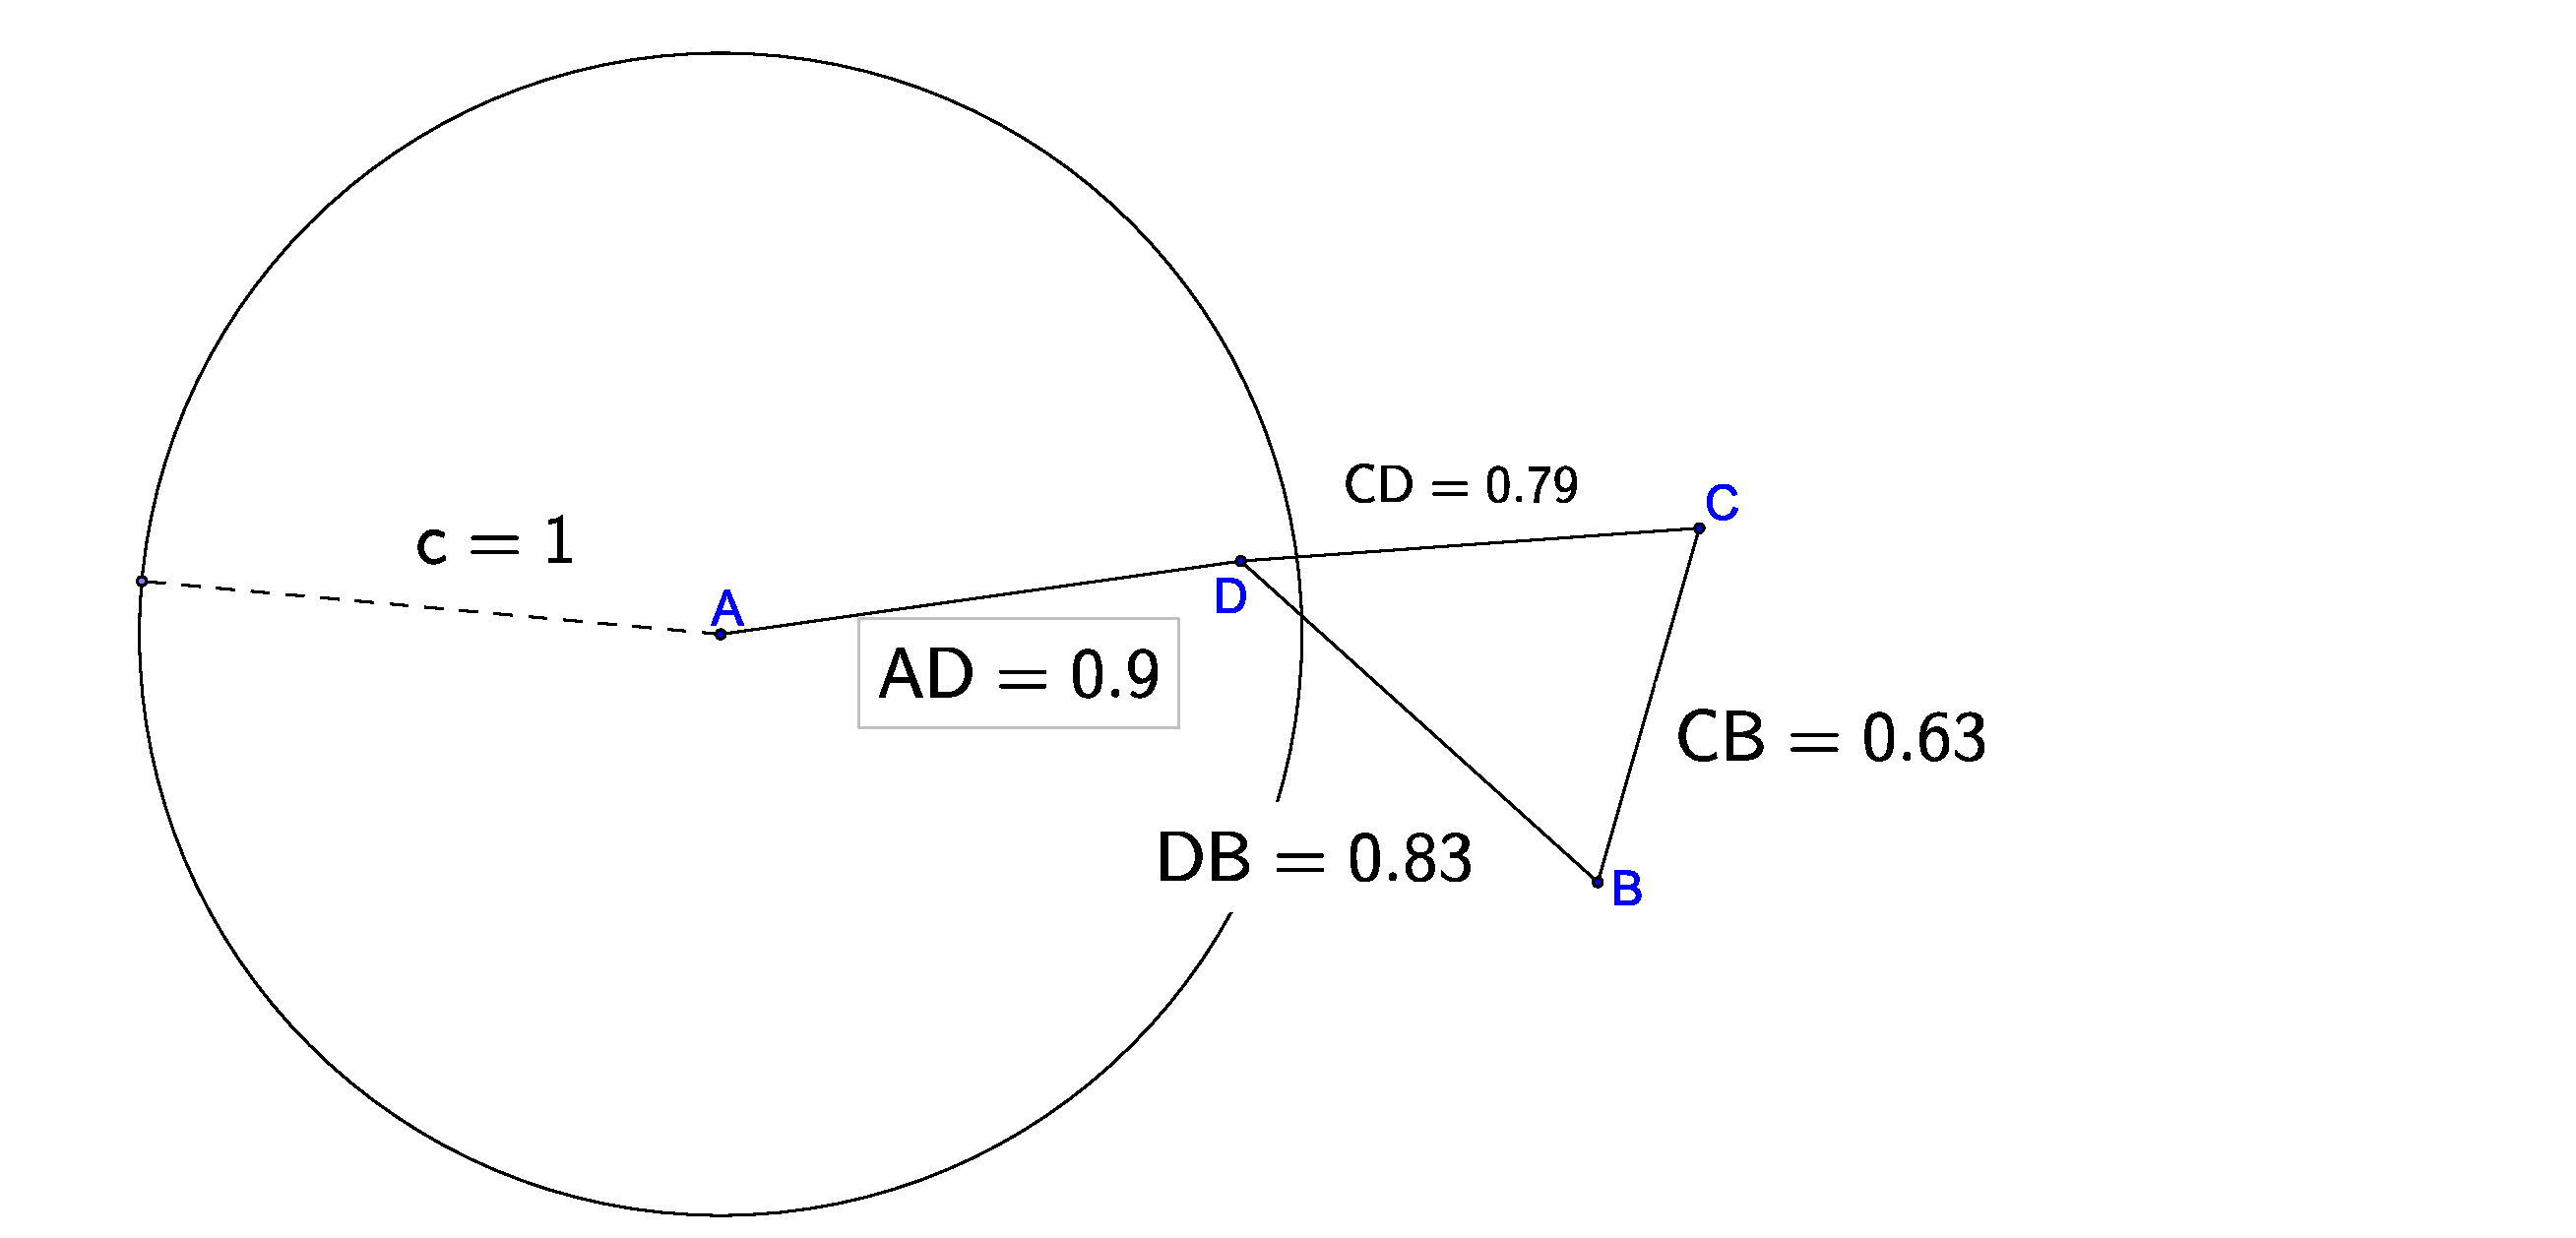
\includegraphics[width=0.99\linewidth]{UnitGraph.eps}
\caption{}
\label{fig:UnitGraph}
\end{figure}



\subsection{Spanner}
Gegeben ist ein Graph $G $, welcher ein Subgraph vom euklidischen Graphen $E $ ist. $G $ enthält alle Knoten von $E $, aber nicht alle Kanten. Die Umwege, die durch das Löschen von Kanten entstehen, dürfen nur um einen konstanten Faktor ansteigen. 

\subsubsection{Hop Spanner}
Die Pfadlänge wird in Hops gemessen. Ein Hop entspricht einen Übergang von Knoten A nach Knoten B, wenn diese in $G $ enthalten sind. Ein Beispiel dazu folgt:
$include Hop_Beispiel $
\subsubsection{Euklidischer Spanner}
$G $ ist genau dann ein euklidischer Spanner von $H $, wenn die kürzesten Pfade zwischen allen Knoten, maximal um einen konstanten Faktor $t $ vergrößert werden:

$c_G(A,B) \leq t \cdot c_H(A,B) $

\subsection{Yao Step}
Gegeben ist ein Graph $G $. Für alle Knoten $A \in G $ wird folgender Algorithmus ausgeführt:
\begin{enumerate}
\item Erzeuge k gleich große Kegel um $A $.
\item Bestimme die kürzeste Kante in jedem Kegel.
\item Lösche alle Kanten, die nicht von beiden Endpunkten ausgewählt wurden.

\end{enumerate} 
%Dadurch entsteht Graph $G' $. 

\subsection{Delaunay Triangulation}
Die Delaunay Triangulation erzeugt aus einem beliebigen zusammenhängenden Graphen einen geometrischen (= euklidischen) Spanner mit dem Streckungsfaktor $c_{del} \approx 2.42 $ und einem beliebig hohen Ausgangsgrad eines Knotens. Dazu werden alle Dreiecke betrachtet. Wenn der Kreis durch alle Eckpunkte des Dreiecks keine weiteren Punkte des Graphen enthält, sind diese drei Kanten auch im Delaunay Graphen.

\subsection{Lokale Algorithmen}
\subsubsection{streng lokal}
\subsubsection{title}


\section{was erreicht diese Arbeit} %bearbeiten

\section{Geometrische Spanner}
\section{Fazit}



\bibliographystyle{IEEEtran}
\bibliography{biblio}

\end{document}
